\chapter{反復最適化}
\label{cha:optimization}

\begin{leadbox}
本章では,与えられたコスト関数を最小化するパラメータを求める問題に対する
反復最適化技法について解説します.
現実の多くの問題では,コスト関数を最小化するパラメータを直接計算することができないため,
パラメータを徐々に変化させることでコスト関数を徐々に小さくしていく方法をとります.
具体的には,一般的なコスト関数最小化(あるいは尤度関数最大化)のアルゴリズムとして,
最急降下法,ニュートン法・準ニュートン法,補助関数法,乗法更新アルゴリズムを紹介します.
また,ベイズモデルの事後分布の計算に用いることができる
変分ベイズ法とマルコフ連鎖モンテカルロ法についても紹介します.
\end{leadbox}

\section{コスト関数最小化}
\label{sec:cost_function_optimizaition}

最初に,コスト関数を最小化する問題を数学的に定義します.
いま,あるパラメータ$\bm{X}$に関するコスト関数$f(\bm{X}) \in \mathbb{R}$が与えられたとします.
パラメータはスカラ,ベクトル,行列,それらの集合など様々な形式をとりえますが,
コスト関数の値は常に実数であるものとします.我々の目的は,
\begin{align}
 \bm{X}^* = \argmin_{\bm{X}} f(\bm{X})
\end{align}
となる最適解$\bm{X}^*$を求めることです.

一般に,関数$f(\bm{X})$は多峰性を持っているので,$f(\bm{X})$が最小値をとる最適解を求めることは容易ではなく,
$f(\bm{X})$が極小値を取る局所解を求めることが現実的な目標となります.
大域的な最適性が保証されるのは,$f(\bm{X})$が凸関数である場合がほとんどです.
以降で紹介する反復最適化技法は,パラメータ$\bm{X}$をなんらかの値に初期化し,
その値を少しずつ変化させていく山登り型 (hill climbing) の
(コスト関数「最小化」という意味では山下り型の)アルゴリズムです(\reffig{fig:hill_climbing}).
そのため,最終的に求まる解が大域的に最適である保証はなく,
初期値依存性があることに注意が必要です.
したがって,なんらかの事前知識が使える場合は,初期値を適切に設定することが
より$f(\bm{X})$を小さくする局所解を探索することにつながります.

\begin{figure}[t]
\centering
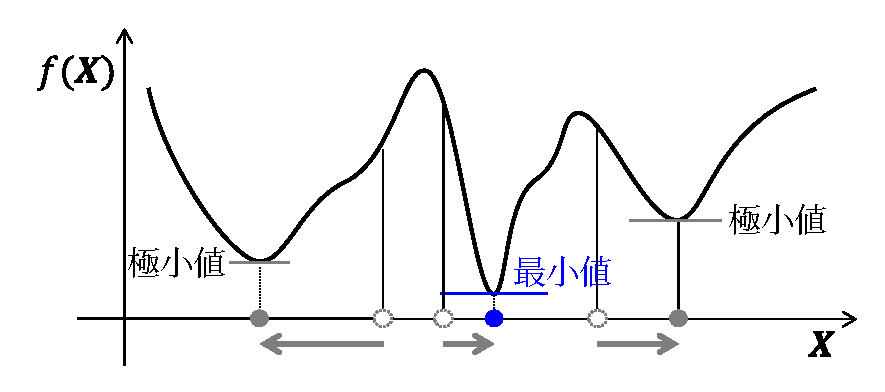
\includegraphics[width=.93\linewidth]{sections/optimization/hill_climbing}
\caption{山登り法(山下り法)による最適解の探索.初期値によっては局所解しか見つからない.}
\label{fig:hill_climbing}
\end{figure}

\subsection{最急降下法}
\label{sec:steepest_descent}

最急降下法 (steepest descent method) はもっとも単純な反復最適化技法で,
コスト関数の勾配方向の逆方向にパラメータを更新します.
本節では,パラメータ$\bm{X}$は,$N$次元ベクトル$\bm{x} = [x_1,\cdots,x_N]^T\in \mathbb{R}^N$であるとします.
このとき,関数$f(\bm{x})$の勾配ベクトル (gradient vector) は
\begin{align}
\nabla f(\bm{x}) = \left[\frac{\partial f(\bm{x})}{\partial x_1},\ldots,\frac{\partial f(\bm{x})}{\partial x_N}\right]^T
\end{align}
で与えられます.このとき,$\nabla f(\bm{x})$は$f(\bm{x})$の等高面,
すなわち,$f(\bm{x})$が一定となるような$N$次元空間内の曲面に対して,
その法線ベクトルを与えます.
このベクトルの向きは,関数の値が増加する方向を示しています.

\begin{algobox}{最急降下法}
\label{algo:steepest}
\begin{algorithmic}[1]
\Require 最小化すべきコスト関数$f(\bm{x}) \in \mathbb{R}$
\State パラメータ$\bm{x} \in \mathbb{R}^N$をランダムに初期化
\While{$\nabla f(\bm{x}) \ne \bm{0}$}
\State 探索ベクトル$d(\bm{x}) = - \nabla f(\bm{x})$を計算
\State ステップ幅$\alpha$を適切に設定
\State $\bm{x} \gets \bm{x} + \alpha d(\bm{x})$
\EndWhile\\
{\bf Return} パラメータ$\bm{x}$
\end{algorithmic}
\end{algobox}

\refalgo{algo:steepest}に,$\bm{x}$を更新するアルゴリズムを示します.
具体的に,$\bm{x} = [x_1,x_2]^T$として$f(\bm{x}) = x_1^2 + x_2^2$の最小化について考えてみます.
このとき,勾配ベクトルは
\begin{align}
 \nabla f(\bm{x}) = [2 x_1, 2 x_2]^T
\end{align}
となるので,ある$\bm{x}$における$\nabla f(\bm{x})$の向きは,原点と$\bm{x}$とを結ぶ方向になります.
この例では,$f(\bm{x})$が一定となる等高線は円であり,
確かに$\nabla f(\bm{x})$は等高線に対する法線ベクトルになっています.
したがって,$\nabla f(\bm{x})$の逆向きの方向が
最も$f(\bm{x})$の値が減少する方向$d(\bm{x})$であるので,
$d(\bm{x})$の方向に沿って$\bm{x}$を「少しずつ」動かせばよいのです.

ここで重要なのは,ステップサイズ$\alpha$の設定です.
$\alpha$を大きくすると,$\bm{x}$は大きく更新されるので,局所解へ早く収束しそうです.
しかし,大きくしすぎると,局所解の周辺をいったりきたりしてしまいます.
そのため,実際には,直線探索を用いて適切な$\alpha$を決定することがよく行われます.
一般には,$\alpha$を少しずつ小さくしていくことが好ましいとされています.

最急降下法は,$f(\bm{x})$が唯一の極小点を持つときには,
停留点($\nabla f(\bm{x}) = 0$となる$\bm{x}$)への大域的な収束性が保証されています.
また,計算量が軽く,実装が簡単ですが,収束が遅いことが欠点です.

\subsection{ニュートン法}
\label{sec:newton}

収束が遅いという最急降下法の欠点を克服する方法として,
ニュートン法 (Newton's method) が知られています.
ニュートン法は,コスト関数$f(\bm{x})$の一次導関数$\nabla f(\bm{x})$だけではなく,
二次導関数$\nabla^2 f(\bm{x})$を利用することで,
探索ベクトル$d(\bm{x})$の計算に工夫を行います.
まず,$f(\bm{x})$に対して,二次のテイラー展開を行うと
\begin{align}
f(\bm{x} + \Delta \bm{x}) 
&\approx f(\bm{x}) + \nabla f(\bm{x})^T \Delta\bm{x}
+ \frac{1}{2} \Delta\bm{x}^T \nabla^2 f(\bm{x}) \Delta\bm{x}
\nonumber\\
&\overset{\mbox{\scriptsize def}}{=} t(\bm{x} + \Delta\bm{x})
\label{eqn:fx_taylor}
\end{align}
を得ます.ここで,二次導関数$\nabla^2 f(\bm{x})$は
\begin{align}
\nabla^2 f(\bm{x}) =
  \begin{bmatrix}
    \displaystyle
    \frac{\partial^2 f(\bm{x})}{\partial x_1 \partial x_1} &
    \cdots&
    \displaystyle
    \frac{\partial^2 f(\bm{x})}{\partial x_1 \partial x_N}\\
    \vdots & & \vdots \\
    \displaystyle
    \frac{\partial^2 f(\bm{x})}{\partial x_N \partial x_1} &
    \cdots& 
    \displaystyle \frac{\partial^2 f(\bm{x})}{\partial x_N \partial x_N}    
  \end{bmatrix}
\end{align}
で与えられます.$\nabla^2 f(\bm{x})$は,関数$f(\bm{x})$のヘッセ行列 (Hessian matrix) とよばれ,
しばしば$H(\bm{x})$と表されます.
$f(\bm{x})$が二階連続微分可能であれば,$H(\bm{x})$は対称行列となります.
\refeq{eqn:fx_taylor}の二次近似の精度が十分によければ,
$t(\bm{x} + \Delta\bm{x})$を最小化する$\Delta\bm{x}$が,
$f(\bm{x} + \Delta\bm{x})$を最小化する$\Delta\bm{x}$のよい近似になっており,
$\bm{x} \gets \bm{x} + \Delta\bm{x}$と更新すればよいことになります.

覚えておくべき重要な性質として,$\bm{x}$が$f(\bm{x})$の極小点をとるには,
ヘッセ行列$H(\bm{x})$は正定値行列である必要があります(必要十分ではありません).
行列の正定値性とは,固有値が全て正であることを意味し,
スカラの正値性を拡張した概念です.
例えば,$N=1$のとき,$f(\bm{x})$はスカラを入力とする関数となり,
その極小点において,一次導関数の値は負から正に切り替わるので,
二次導関数の値は正をとらなくてはなりません.
$N > 1$のときは,$f(\bm{x})$はベクトルを入力とする関数であり,
二次導関数は行列形式で与えられます.
このとき,極小点において,
スカラの正値性を多次元拡張した性質である半正定値性が成立することになります.

ヘッセ行列$H(\bm{x})$が正定値であるとして,
\refeq{eqn:fx_taylor}に対して平方完成を行うと,$\Delta\bm{x}$の二次関数
\begin{align}
t(\bm{x} &+ \Delta\bm{x}) 
= f(\bm{x}) - \frac{1}{2} \nabla f(\bm{x})^T H(\bm{x})^{-1} \nabla f(\bm{x}) 
\nonumber\\
&+ \frac{1}{2} \left(\Delta\bm{x} + H(\bm{x})^{-1} \nabla f(\bm{x})\right)^T H(\bm{x}) \left(\Delta\bm{x} + H(\bm{x})^{-1} \nabla f(\bm{x})\right)
\end{align}
を得ます.この二次関数は,
\begin{align}
 \Delta\bm{x} = - H(\bm{x})^{-1} \nabla f(\bm{x})
 \label{eqn:xi_h_n}
\end{align}
のとき最小値をとります.
したがって,$\bm{x} \gets \bm{x} - H(\bm{x})^{-1} \nabla f(\bm{x})$とすることで
$f(\bm{x})$を効率的に小さくすることができるはずです.

\begin{algobox}{ニュートン法}
\label{algo:newton}
\begin{algorithmic}[1]
\Require 最小化すべきコスト関数$f(\bm{x}) \in \mathbb{R}$
\State パラメータ$\bm{x} \in \mathbb{R}^N$をランダムに初期化
\While{$\nabla f(\bm{x}) \ne \bm{0}$}
\State 探索ベクトル$d(\bm{x}) = - \left(\nabla^2 f(\bm{x})\right)^{-1} \nabla f(\bm{x})$を計算
\State ステップ幅$\alpha$を適切に設定
\State $\bm{x} \gets \bm{x} + \alpha d(\bm{x})$
\EndWhile\\
{\bf Return} パラメータ$\bm{x}$
\end{algorithmic}
\end{algobox}

\refalgo{algo:newton}に,$\bm{x}$を更新するアルゴリズムを示します.
$f(\bm{x})$が二次関数である場合には,\refeq{eqn:fx_taylor}の近似で誤差は生じないため,
\refeq{eqn:xi_h_n}のときに$f(\bm{x} + \Delta\bm{x})$は最小値をとり,反復は一回で終了します.
実際には,$f(\bm{x})$は二次関数でない場合が普通であり,
探索ベクトル$d(\bm{x})$の方向に$1$以外のスケールで動かせるようにステップ幅$\alpha$が導入されています.

ニュートン法は収束速度が速いですが,
初期値が局所解に十分に近くないと収束性が保証されません.
ただし,実用上は,$\alpha=1$としても問題なく収束する場合が多いです.
また,特に$N$が大きい場合に問題となりますが,数値的に不安定になりやすく,
ヘッセ行列$H(\bm{x})$が正定値性を満たさなくなったり,
逆行列$H(\bm{x})^{-1}$の計算負荷が大きいといった欠点があります.

\subsection{準ニュートン法}
\label{sec:quasi_newton}

ヘッセ行列$H(\bm{x})$やその逆行列を直接計算しなければならないというニュートン法の欠点を克服するため,
準ニュートン法 (quasi-Newton method) が知られています.
準ニュートン法では,最適化の繰り返し計算の過程で得られる勾配ベクトルにより,
ヘッセ行列$H(\bm{x})$の近似を行います.
まず,(精度はともかく)勾配ベクトルは次式で近似できます.
\begin{align}
 \nabla f(\bm{x} + \Delta\bm{x}) \approx \nabla f(\bm{x}) + H(\bm{x})\Delta\bm{x}
\end{align}
したがって,$H(\bm{x})$の近似値として,セカント方程式 (Secant equation)
\begin{align}
 \nabla f(\bm{x} + \Delta\bm{x}) = \nabla f(\bm{x}) + B(\bm{x})\Delta\bm{x}
\end{align}
を満たすような$B(\bm{x})$を求めればよいことになります.

\begin{algobox}{準ニュートン法}
\label{algo:quasi_newton}
\begin{algorithmic}[1]
\Require 最小化すべきコスト関数$f(\bm{x}) \in \mathbb{R}$
\State パラメータ$\bm{x} \in \mathbb{R}^N$をランダムに初期化
\State 近似ヘッセ行列$B(\bm{x})$を初期化(単位行列など)
\While{$\nabla f(\bm{x}) \ne \bm{0}$}
\State 探索ベクトル$d(\bm{x}) = - B(\bm{x})^{-1} \nabla f(\bm{x})$を計算
\State ステップ幅$\alpha$を適切に設定
\State $\bm{x}$の変化量$\Delta\bm{x} = \alpha d(\bm{x})$を計算
\State $\nabla f(\bm{x})$の変化量$\bm{y} = \nabla f(\bm{x} + \Delta\bm{x}) - \nabla f(\bm{x})$を計算
\State $\bm{x} \gets \bm{x} + \Delta\bm{x}$
\State 近似ヘッセ行列の逆行列$B(\bm{x})^{-1}$を更新
\EndWhile\\
{\bf Return} パラメータ$\bm{x}$
\end{algorithmic}
\end{algobox}

\refalgo{algo:quasi_newton}に,$\bm{x}$を更新するアルゴリズムを示します.
準ニュートン法では,パラメータ$\bm{x}$だけではなく,
近似ヘッセ行列$B(\bm{x})$も反復的に更新されるため,
両者を初期化しておく必要があります.
\reftab{tab:hessian_update}および\reftab{tab:inv_hessian_update}に,
近似ヘッセ行列$B(\bm{x})$あるいはその逆行列$C(\bm{x}) = B(\bm{x})^{-1}$を求めるアルゴリズムを示します.
最初のアルゴリズムであるDFP法は,最近はあまり用いられていません.
現在最も用いられているアルゴリズムは,
BFGS法 (提案者であるBroyden, Fletcher, Goldfarb, Shannoの頭文字から) とSR1法です.
準ニュートン法を大規模問題に応用するため,
記憶制限準ニュートン法 (limited-memory quasi-Newton method) が発表され,
BFGS法の記憶制限版としてL-BFGS法が盛んに利用されています.
SR1法は,ヘッセ行列の更新時に正定値性が保存されないため,
不定値行列に対しても用いることができます.
また,Broyden法は行列が対称行列でなくとも良く,
通常の連立方程式の解を求めるのにも使うことができます.

\begin{table}[t]
\centering
\caption{近似ヘッセ行列$B(\bm{x})$の更新}
\label{tab:hessian_update}
\begin{tabular}{l|l}
\hline
手法 & 更新式
\\
\hline
DFP 
&
$\displaystyle B(\bm{x}) \gets \left (I-\frac {\bm{y} \, \Delta\bm{x}^T} {\bm{y}^T \, \Delta\bm{x}} \right ) B(\bm{x}) \left (I-\frac {\Delta\bm{x} \bm{y}^T} {\bm{y}^T \, \Delta\bm{x}} \right )+\frac{\bm{y} \bm{y}^T} {\bm{y}^T \, \Delta\bm{x}}$
\\
BFGS
&
$\displaystyle B(\bm{x}) \gets B(\bm{x}) + \frac {\bm{y} \bm{y}^T}{\bm{y}^{T} \Delta\bm{x}} - \frac {B(\bm{x}) \Delta\bm{x} (B(\bm{x}) \Delta\bm{x})^T} {\Delta\bm{x}^{T} B(\bm{x}) \, \Delta\bm{x}}$
\\
SR1
&
$\displaystyle B(\bm{x}) \gets B(\bm{x}) +\frac {(\bm{y}-B(\bm{x}) \, \Delta\bm{x}) (\bm{y}-B(\bm{x}) \, \Delta\bm{x})^T}{(\bm{y}-B(\bm{x}) \, \Delta\bm{x})^T \, \Delta\bm{x}}$
\\
Broyden
&
$\displaystyle B(\bm{x}) \gets B(\bm{x})+\frac {\bm{y}-B(\bm{x}) \Delta\bm{x}}{\Delta\bm{x}^T \, \Delta\bm{x}} \, \Delta\bm{x}^T$
\\
\hline
\end{tabular}
\end{table}

\begin{table}[t]
\centering
\caption{近似ヘッセ行列の逆行列$C(\bm{x}) = B(\bm{x})^{-1}$の更新}
\label{tab:inv_hessian_update}
\begin{tabular}{l|l}
\hline
手法 & 更新式
\\
\hline
DFP 
&
$\displaystyle C(\bm{x}) \gets \displaystyle C(\bm{x}) + \frac {\Delta\bm{x} \Delta\bm{x}^T}{\bm{y}^{T} \, \Delta\bm{x}} - \frac {C(\bm{x}) \bm{y} \bm{y}^T C(\bm{x})^T} {\bm{y}^T C(\bm{x}) \bm{y}}$
\\
BFGS
&
$\displaystyle C(\bm{x}) \gets \left (I-\frac {\bm{y} \Delta\bm{x}^T} {\bm{y}^T \Delta\bm{x}} \right )^T C(\bm{x}) \left (I-\frac { \bm{y} \Delta\bm{x}^T} {\bm{y}^T \Delta\bm{x}} \right )+\frac
{\Delta\bm{x} \Delta\bm{x}^T} {\bm{y}^T \, \Delta\bm{x}}$
\\
SR1
&
$\displaystyle C(\bm{x}) \gets C(\bm{x})+\frac {(\Delta\bm{x}-C(\bm{x}) \bm{y}) (\Delta\bm{x}-C(\bm{x}) \bm{y})^T}{(\Delta\bm{x}-C(\bm{x}) \bm{y})^T \bm{y}}$
\\
Broyden
&
$\displaystyle C(\bm{x}) \gets C(\bm{x})+\frac {(\Delta\bm{x}-C(\bm{x}) \bm{y}) \Delta\bm{x}^T C(\bm{x})}{\Delta\bm{x}^T C(\bm{x}) \, \bm{y}}$
\\
\hline
\end{tabular}
\end{table}

\subsection{補助関数法}
\label{sec:auxiliary_function}

これまで紹介してきた汎用的な最適化技法とは異なり,
ある条件下において収束性の保証された更新則を導出できる補助関数法を紹介します.
この方法では,それほど簡単ではないステップ幅を設定する必要がなく,
経験的には高速に収束することが知られています.

\begin{algobox}{補助関数法}
\label{algo:aux_function}
\begin{algorithmic}[1]
\Require 最小化すべきコスト関数$f(\bm{X}) \in \mathbb{R}$
\State 補助変数$\bm\Theta$を導入して,上限関数$u(\bm{X}, \bm\Theta) \in \mathbb{R}$を設計
\State パラメータ$\bm{X}$をランダムに初期化
\While{$u(\bm{X}, \bm\Theta)$の変化量が大きい}
\State $\bm\Theta \gets \argmin_{\bm\Theta} u(\bm{X}, \bm\Theta)$
\State $\bm{X} \gets \argmin_{\bm{X}} u(\bm{X}, \bm\Theta)$
\EndWhile\\
{\bf Return} パラメータ$\bm{X}$
\end{algorithmic}
\end{algobox}

\refalgo{algo:aux_function}に,$\bm{X}$を更新するアルゴリズムを示します.
ここでは,$\bm{X}$はベクトルに限定せず,任意の形式をとるものとします.
補助関数法では,コスト関数$f(\bm{X})$の上限関数$u(\bm{X}, \bm\Theta)$を設計し,
$\bm{X}$と$\bm\Theta$について交互に$u(\bm{X}, \bm\Theta)$を逐次最小化することで,
間接的に$f(\bm{X})$を逐次最小化します.
ここで,$\bm\Theta$は新たに導入された補助変数で,
$u(\bm{X}, \bm\Theta)$を$\bm\Theta$について最小化すると,
もとの関数$f(\bm{X})$と同じ値をとるようにしておきます.
\begin{align}
f(\bm{X}) = \min_{\bm\Theta} u(\bm{X},\bm\Theta)
\end{align}

このアルゴリズムの収束性を証明します.
いま,あるステップ$k$における$\bm{X}$および$\bm\Theta$の値を
$\bm{X}^{(k)}$および$\bm\Theta^{(k)}$とすると,
上限関数の性質から
\begin{align}
f(\bm{X}^{(k)}) 
&= \min_{\bm\Theta} u(\bm{X}^{(k)},\bm\Theta) = u(\bm{X}^{(k)},\bm\Theta^{(k + 1)})
\nonumber\\
&\ge u(\bm{X}^{(k + 1)},\bm\Theta^{(k + 1)})
\nonumber\\
&\ge u(\bm{X}^{(k + 1)},\bm\Theta^{(k + 2)})
= f(\bm{X}^{(k + 1)})
\end{align}
となります(\reffig{fig:aux_function}).
したがって,$\{f(\bm{X}^{(k)})\}_{k=1}^\infty$は単調非増加 (monotonically non-increasing) となり,
停留点に収束します.

\begin{figure}[t]
\centering
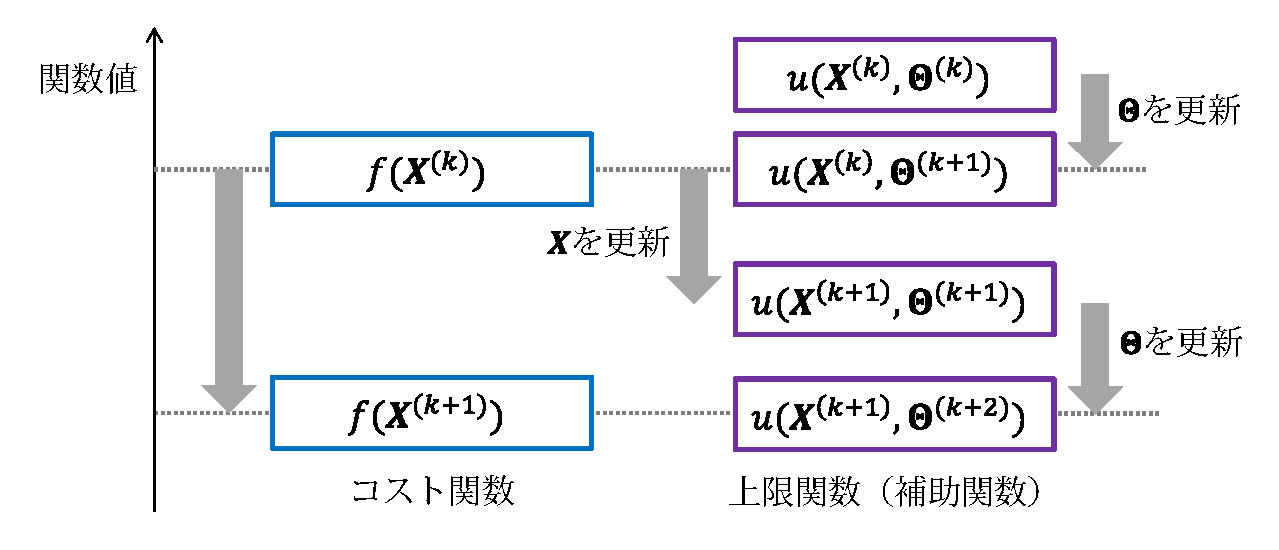
\includegraphics[width=.98\linewidth]{sections/optimization/aux_function}
\vspace{-1mm}
\caption{補助関数法によるパラメータ$\bm{X}$と補助変数$\bm\Theta$の反復最適化.}
\label{fig:aux_function}
\end{figure}

補助関数法の肝は,$f(\bm{X})$を直接最小化することは困難であるものの,
一方の変数の値が既知であれば,もう一方の変数について最小化することが容易になるような
$u(\bm{X}, \bm\Theta)$をうまく設計することにあります.
例えば,$u(\bm{X}, \bm\Theta)$が$\bm{X}$に関する凸関数となっており,
$\bm{X}$で偏微分してゼロとおいた式が解析的に解けるとすると,
$\bm\Theta$が与えられたもとでの$\bm{X}$の最適解を得ることができます.
このとき,アルゴリズムは高速に収束することが期待できます.

最適化を行いやすい$u(\bm{X}, \bm\Theta)$を設計するうえで有用な基本原理について説明します.
まず,$f$が凸関数 (convex function) である場合,
イェンセンの不等式 (Jensen's inequality) が適用できる可能性があります.
\begin{theobox}{イェンセンの不等式}
\label{jensen}
任意の凸関数$f:\mathbb{R}^N \rightarrow \mathbb{R}$に対して,
\begin{align}
f\left(\sum_{k=1}^K \lambda_k \bm{x}_k\right) \le \sum_{k=1}^K \lambda_k f(\bm{x}_k)
\end{align}
が成立します.
ただし,$\{\bm{x}_k\}_{k=1}^K$は任意の$N$次元ベクトルで,
$\{\lambda_k\}_{k=1}^K$は$\lambda_k \ge 0$かつ$\sum_{k=1}^K \lambda_k = 1$を満たす非負の実数です.
\end{theobox}
これが成立することは,凸関数の定義からほぼ明らかです.
\reffig{fig:aux_function_conv_concave}(a)に,
$N=1$であるときのイェンセンの不等式の様子を示します.
不等式の左辺は,$\{\bm{x}_k\}_{k=1}^K$の重み付き和をとってから関数値を計算していますが,
右辺は,各$\bm{x}_k$における関数値を計算してから,重み付き和をとっています.
したがって,$f$が凸関数であるならば,後者の方が大きくなります.
例えば,凸関数$f(x) = - \log (x)$に対して,以下のように用います.
\begin{align}
- \log \left(\sum_{k=1}^K \lambda_k x_k\right) \le - \sum_{k=1}^K \lambda_k \log (x_k)
\end{align}

一方,$f$が凹関数 (concave function) である場合,
一次のテイラー展開に基づく接平面を補助関数に用いることができます.
\begin{theobox}{接平面に基づく不等式}
\label{jensen}
任意の凹関数$f:\mathbb{R}^N \rightarrow \mathbb{R}$に対して,
\begin{align}
f(\bm{x}) \le f(\bm\omega) + f'(\bm\omega)^T(\bm{x} - \bm\omega)
\end{align}
が成立します.ただし,$\bm{x}$および$\bm\omega$は任意の$N$次元ベクトルです.\\[-4mm]
\end{theobox}
\reffig{fig:aux_function_conv_concave}(b)に,
$N=1$であるときのの不等式の様子を示します.
不等式の右辺は,$\bm{x}$の一次式であるので,
$N=1$のときは接平面の方程式を表します.
例えば,凹関数$f(x) = \log (x)$に対して,以下のように用います.
\begin{align}
\log(x) \le \log(\omega) + \frac{1}{\omega}(x - \omega) = \frac{x}{\omega} + \log(\omega) - 1
\end{align}

\begin{figure}[t]
\centering
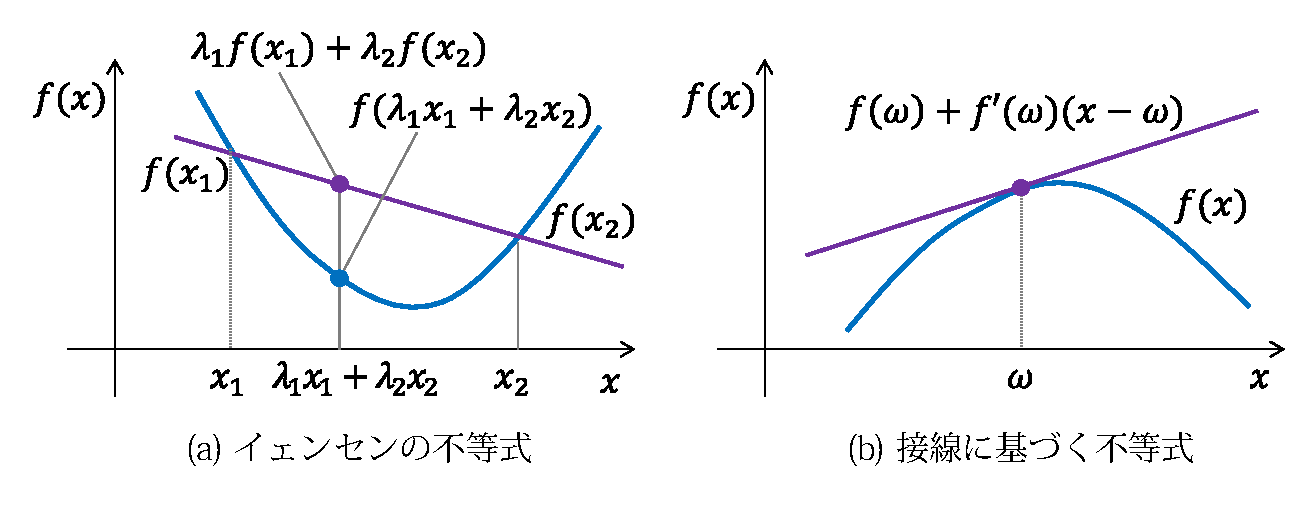
\includegraphics[width=.98\linewidth]{sections/optimization/aux_function_conv_concave}
\vspace{-2mm}
\caption{コスト関数の上限関数を導出するうえで有用な基本原理.}
\label{fig:aux_function_conv_concave}
\end{figure}

\subsection{乗法更新アルゴリズム}
\label{sec:multiplicative_update}

コスト関数$f(\bm{X})$の入力$\bm{X}$が非負値のスカラ$x$である場合には,
乗法更新アルゴリズムと呼ばれる反復最適化技法が利用できる場合があります.
この手法では,特別な制約を導入しなくても,
毎回の反復における$x$の非負値性を自然に保つことができます.

まず,一般的な乗法更新則の導出方法をまとめておきます.
いま,ある変数$x$に関するコスト関数$f(x)$が与えられており,
これを$x$について最小化する問題を考えます.
このとき,$f(x)$の$x$に関する一次導関数が
\begin{align}
\frac{\partial f(x)}{\partial x} = \kappa^+(x) - \kappa^-(x)
\end{align}
の形で表現できたとします.
ただし,$\kappa^+(x) > 0$および$\kappa^-(x) > 0$は
$x$の関数であり,常に正をとるものとします.
このとき,
\begin{align}
x \gets \frac{\kappa^-(x)}{\kappa^+(x)} x
\end{align}
とすると,$f(x)$が小さくなることが期待できます.
収束性は理論的に保証されていませんが,実用上は問題がない場合が多いです.

\begin{figure}[t]
\centering
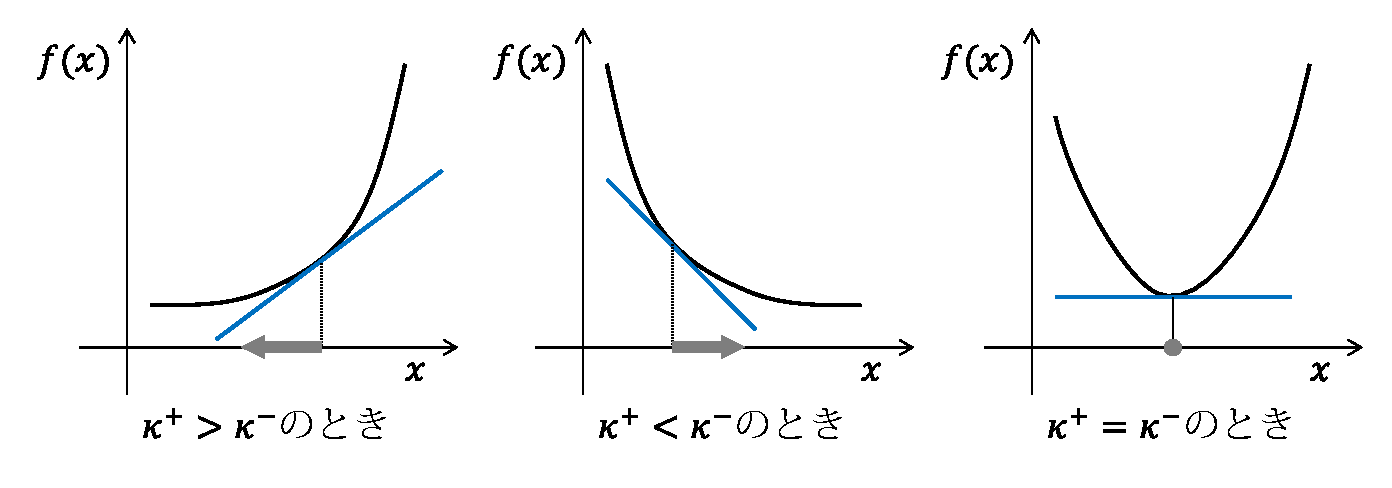
\includegraphics[width=.99\linewidth]{sections/optimization/multiplicative_update}
\caption{$f(x)$の最小化に乗法更新則を適用した場合の$x$の変化.}
\label{fig:multiplicative_update}
\end{figure}

このアルゴリズムが$f(x)$の値を小さくすることができるのかについて,
$\kappa^+$および$\kappa^-$の大小関係で場合分けして考察してみます(\reffig{fig:multiplicative_update}).
\begin{itemize}
\item
$\kappa^+ > \kappa^-$のとき:\\
$\frac{\partial f(x)}{\partial w} > 0$となり,
$f(x)$の$w$に関する傾きは正であるので,
$f(x)$を小さくするには,$w$を小さくする必要があります.
\refeq{eqn:mu_eta_km}をみると,分子より分母の方が大きくなるため,$\eta < 1$であり,
$w \gets \eta w$とすると,$w$を小さくできます.
\item
$\kappa^+ < \kappa^-$のとき:\\
$\frac{\partial f(x)}{\partial w} < 0$となり,
$f(x)$の$w$に関する傾きは負であるので,
$\eta > 1$とすることで,$w$を大きくします.
\item
$\kappa^+ = \kappa^-$のとき:\\
$\frac{\partial f(x)}{\partial w} = 0$となり,
$f(x)$は$w$において停留点をとることを示しています.
そのため,$\eta = 1$とすることで,$w$の更新を行わないようにします.
\end{itemize}

\section{確率モデルの最適化}

本節では,確率モデルを用いて推論を行う上で必要となる最適化技法について紹介します.
観測データが与えられた時に,
確率モデルのパラメータを推定するには,主に3つのアプローチがあります.
いま,確率モデルのパラメータを$\bm\theta$,
その確率モデルから生成された観測データを$\bm{X}$とします.
\begin{description}
\item[最尤推定 (maximum-likelihood (ML) estimation)] \ \\
最尤推定では,パラメータ$\bm\theta$の尤度関数$f(\bm\theta) = p(\bm{X}|\bm\theta)$を
最大化するような$\bm\theta^*$を点推定する(一意に決定する)ことが目標です.
\begin{align}
\bm\theta^* = \argmax_{\bm\theta} p(\bm{X}|\bm\theta)
\end{align}
ここで,$p(\bm{X}|\bm\theta)$は,$\bm\theta$から$\bm{X}$が生成される
確率\footnote{連続側の分布の場合,正確には確率密度ですが,
本書では区別せずに「確率」と呼びます.}を表すので,
この値が大きい$\bm\theta$ほど尤もらしいと考えます.
尤度関数はコスト関数の一種であるので,導関数を計算するなどして最適解が解析的に求められない場合は,
これまで説明してきた反復最適化技法を利用することができます.
最尤推定は幅広く用いられている最も標準的なアプローチですが,
観測データ$\bm{X}$があまり大きくない場合には,
推定結果が不正確になりやすい問題があります.
なぜなら,パラメータの値は観測データ$\bm{X}$のみによって決まり,
(もしあれば)パラメータの値としてありえそうな範囲に関する事前知識が
反映されていないからです.

\item[最大事後確率推定 (maximum-a-posteriori (MAP) estimation)] \ \\
MAP推定では,パラメータ$\bm\theta$に対する事前分布$p(\bm\theta)$を導入し,
事前分布$p(\bm\theta)$と尤度関数$p(\bm{X}|\bm\theta)$との積を
最大化するような$\bm\theta^*$を点推定することが目標です.
\begin{align}
\bm\theta^* = \argmax_{\bm\theta} p(\bm{X}|\bm\theta) p(\bm\theta)
\end{align}
ただし,MAP推定では,事前知識を反映して,$p(\bm\theta)$を適切に設定する必要があります.
もし,$\bm\theta$の取りうる値が広範囲にわたっている場合はなだらかな確率分布を,
$\bm\theta$がある特定の値の近くを取ることが分かっている場合は急峻な確率分布を設定します.
これにより,事前知識\footnote{「仮想的な」観測データと解釈することができます.
多くの場合,$p(\bm\theta)$には仮想的な観測データの個数と解釈できるパラメータが含まれており,
パラメータ推定時に事前分布をどの程度重視するかを自由に制御することができます.}と
実際の観測データとを考慮することで,
観測データが小さい場合でも,事前知識に基づく安定したパラメータ推定が可能になります.
事前分布が一様分布の場合(事前知識が特にない場合),MAP推定は最尤推定と同じ結果を与えます.
MAP推定においても,最尤推定と同様に,標準的な方法を用いた最適化が可能です.

\item[ベイズ推定 (Bayesian estimation)] \ \\
最尤推定・MAP推定では,パラメータ$\bm\theta$を点推定していたのに対し,
ベイズ推定では,ベイズの定理を用いることで,
事前分布$p(\bm\theta)$と尤度関数$p(\bm{X}|\bm\theta)$から
事後分布$p(\bm\theta|\bm{X})$を求めることが目標です.
\begin{align}
 p(\bm\theta|\bm{X}) = \frac{p(\bm{X}|\bm\theta)p(\bm\theta)}{p(\bm{X})}
\end{align}
本来,$\bm\theta$は未知ですから,その推定結果には不確実性が伴います.
したがって,観測データが十分にない場合には,
100\%の確信度をもって$\bm\theta$の値を一意に決めることは難しいのです.
このような場合には特に,
$\bm\theta$のあらゆる可能性を考慮しておくことが望ましいでしょう.
ベイズ推定では,$\bm\theta$の取りうる値それぞれについて,
それがどの程度尤もらしいかという確信度,すなわち確率値を計算します.

現実の多くの問題においては,
周辺尤度$p(\bm{X})=\int p(\bm{X}|\bm\theta) p(\bm\theta) d\bm\theta$を解析的に計算することは困難で
(事後分布$p(\bm\theta|\bm{X})$を解析的に計算できない),何らかの近似推論法が必要になります.
主なものに,\secref{sec:vb}で説明する変分ベイズ法 (variational Bayesian (VB) methods) と
\secref{sec:mcmc}で説明するマルコフ連鎖モンテカルロ法 (Markov chain Monte Carlo (MCMC) methods) が知られており,
いずれも反復計算を行うことにより,事後分布$p(\bm\theta|\bm{X})$を近似する最適化技法です.
\end{description}

\subsection{潜在変数モデル}

\begin{figure}[t]
\centering
\begin{minipage}{.355\linewidth}
\centering
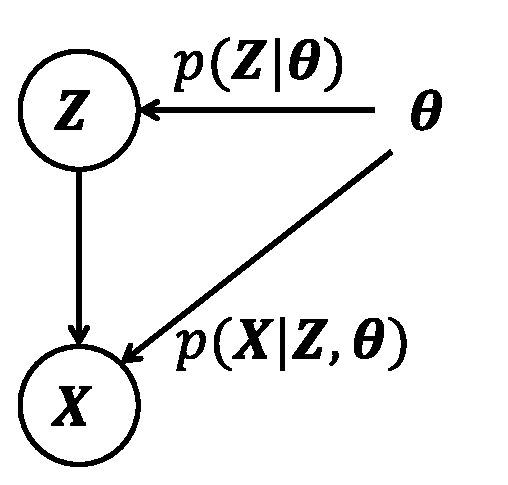
\includegraphics[width=.99\linewidth]{sections/optimization/model_ml}
\caption{確率モデル.}
\label{fig:model_ml}
\end{minipage}
\hspace{6pt}
\begin{minipage}{.56\linewidth}
\centering
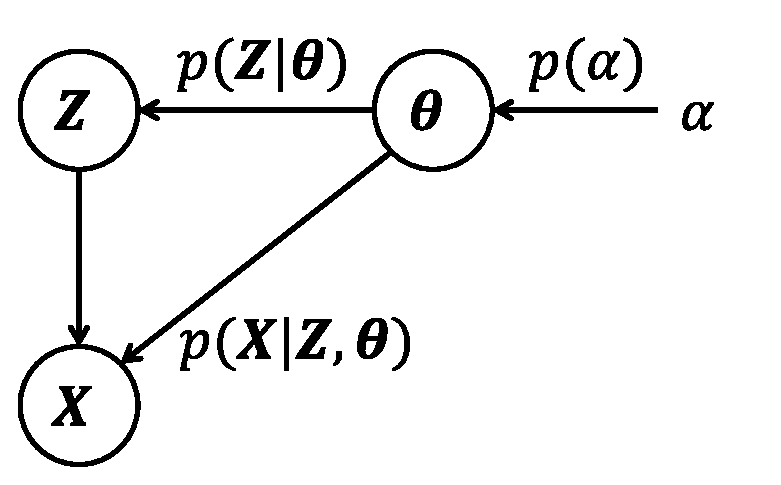
\includegraphics[width=.99\linewidth]{sections/optimization/model_bayes}
\caption{パラメータのベイズ的な取り扱い.}
\label{fig:model_bayes}
\end{minipage}
\end{figure}

現実の多くの問題においては,潜在変数モデルと呼ばれる確率モデルを用いる必要があります.
潜在変数モデルでは,パラメータ$\bm\theta$に加えて,観測変数$\bm{X}$の背後に潜在変数$\bm{Z}$を考えます.
すなわち,以下の生成モデル
\begin{align}
p(\bm{X},\bm{Z},\bm\theta) = p(\bm{X}|\bm{Z},\bm\theta) p(\bm{Z} | \bm\theta)
\end{align}
を考えます.
あとで説明するベイズモデルでは,パラメータ$\bm\theta$も潜在変数$\bm{Z}$も未知であるので,
これらの不確実性を同様に取り扱います.
\begin{align}
p(\bm{X},\bm{Z},\bm\theta) = p(\bm{X}|\bm{Z},\bm\theta) p(\bm{Z} | \bm\theta) p(\bm\theta)
\end{align}

\subsection{EMアルゴリズム}

\subsection{変分ベイズ法}
\label{sec:vb}

\begin{figure}[t]
\centering
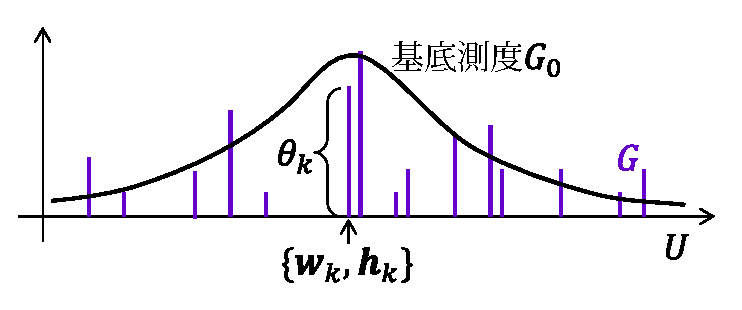
\includegraphics[width=.8\linewidth]{sections/music/gap}
\caption{NMFのためのガンマ過程事前分布.}
\label{fig:gap}
\end{figure}

前節の議論を踏まえて,\refeq{eqn:kl_s_p}, (\ref{eqn:p_w_km}),
(\ref{eqn:p_h_kn}), (\ref{eqn:p_t_k})で定義される
ノンパラメトリックベイズKL-NMF (GaP-KL-NMF)
あるいは\refeq{eqn:is_s_p}, (\ref{eqn:p_w_km}),
        (\ref{eqn:p_h_kn}), (\ref{eqn:p_t_k})で定義される
ノンパラメトリックベイズIS-NMF (GaP-IS-NMF)に対する
変分ベイズ法 (Variational Bayes: VB) について述べる.
今,観測データ$\bm{X}$が与えられたときに,
ベイズの定理を用いて未知パラメータ$\bm\theta,\bm{W},\bm{H}$の事後分布
\begin{eqnarray}
 p(\bm\theta,\bm{W},\bm{H} | \bm{X}) 
 = \frac{p(\bm{X}, \bm\theta,\bm{W},\bm{H})}{p(\bm{X})}
\end{eqnarray}
を計算したい.
しかし,周辺尤度$p(\bm{X})$は解析的に計算できないため,
対数周辺尤度の変分下限$\mathcal{L}(q)$を構成し,
逐次最大化を行うことで$p(\bm{X})$を近似することを考える.
すなわち,変分分布$q(\bm\theta,\bm{W},\bm{H})$に対し,
凹関数$f(x)=\log(x)$に対してJensenの不等式を用いると以下を得る.
\begin{align}
&
 \log p(\bm{X})
 \nonumber\\
&
 = \log \int q(\bm\theta,\bm{W},\bm{H}) 
 \frac{p(\bm{X},\bm\theta,\bm{W},\bm{H})}{q(\bm\theta,\bm{W},\bm{H})} d\bm\theta d\bm{W} d\bm{H}
 \nonumber\\
&
 \ge \int q(\bm\theta,\bm{W},\bm{H}) 
 \log \frac{p(\bm{X},\bm\theta,\bm{W},\bm{H})}{q(\bm\theta,\bm{W},\bm{H})} d\bm\theta d\bm{W} d\bm{H}
 \nonumber\\
&
 = \mathbb{E}_{q(\bm\theta,\bm{W},\bm{H})}[\log p(\bm{X},\bm\theta,\bm{W},\bm{H})]
 \nonumber\\
& \ \ \ \
 - \mathbb{E}_{q(\bm\theta,\bm{W},\bm{H})}[\log q(\bm\theta,\bm{W},\bm{H})]
 \nonumber\\
&
 \overset{\mbox{\scriptsize def}}{=} \mathcal{L}(q)
\end{align}
等号成立条件は$q(\bm\theta,\bm{W},\bm{H}) = p(\bm\theta,\bm{W},\bm{H}|\bm{X})$であり,
このとき$\mathcal{L}(q)$が最大値をとる.
しかし,真の事後分布$p(\bm\theta,\bm{W},\bm{H} | \bm{X})$は計算困難であるため,
変分事後分布を因子分解可能な形$q(\bm\theta,\bm{W},\bm{H}) = q(\bm\theta) q(\bm{W}) q(\bm{H})$に限定し,
その中でも以下で計算できる変分下限
\begin{align}
&
 \mathcal{L}(q) = \mathbb{E}_{q}[\log p(\bm{X}|\bm\theta,\bm{W},\bm{H})]
 + \mathbb{E}_{q}[\log p(\bm\theta)]
 \nonumber\\
& \ \ \ \
 + \mathbb{E}_{q}[\log p(\bm{W})]
 + \mathbb{E}_{q}[\log p(\bm{H})]
 \nonumber\\
& \ \ \ \
 + H(q(\bm\theta)) + H(q(\bm{W})) + H(q(\bm{H}))
 \label{eqn:lb}
\end{align}
を最大化するものを求めたい.
ここで,$H(\cdot)$はエントロピーを表す.
これは,変分事後分布$q(\bm\theta) q(\bm{W}) q(\bm{H})$の
真の事後分布$p(\bm\theta,\bm{W},\bm{H}|\bm{X})$に対するKLダイバージェンスを最小化することと等価である.
\refeq{eqn:lb}を逐次最大化するには,
以下の更新式を収束するまで繰り返せば良い.
\begin{eqnarray}
 \!\!
 q(\bm\theta) \propto \exp(\mathbb{E}_{q(\bm{H},\bm{W})}[\log p(\bm{X},\bm\theta,\bm{W},\bm{H})])
 \label{eqn:q_t}
 \\
 \!\!
 q(\bm{H}) \propto \exp(\mathbb{E}_{q(\bm\theta,\bm{W})}[\log p(\bm{X},\bm\theta,\bm{W},\bm{H})])
 \label{eqn:q_w}
 \\
 \!\!
 q(\bm{W}) \propto \exp(\mathbb{E}_{q(\bm\theta,\bm{H})}[\log p(\bm{X},\bm\theta,\bm{W},\bm{H})]) 
 \label{eqn:q_h}
\end{eqnarray}

\subsection{マルコフ連鎖モンテカルロ法}
\label{sec:mcmc}

MCMCは本来,事後分布$p(\bm\theta|\bm{X})$に従う$\bm\theta$のサンプルを生成するアルゴリズムで,
無限のサンプルを生成できれば,$\bm\theta$の定義域全体からのサンプルを得ることができます.

\subsection{経験ベイズ法}

\section{ベイズ最適化}

